% Johnsongrass life-cycle flow charts
\documentclass[tikz]{standalone}

\usepackage{times}
\usepackage[titletoc]{appendix}
\usepackage{graphicx}
\usepackage{lineno}
\usepackage{multirow}
\usepackage[english]{babel}
\usepackage{typearea} 
\usepackage{amssymb}
\usepackage{amsfonts}
\usepackage{amsmath}
\usepackage{enumerate}
\usepackage{mathtools}
\usepackage{graphicx}
\usepackage{wrapfig}
\usepackage{lscape}
\usepackage{setspace}
\usepackage{rotating}
\usepackage{pdfpages}
\usepackage{pgf}
\usepackage{tikz}
\usepackage{tikzscale}
\usepackage[utf8]{inputenc}
\usetikzlibrary{arrows,automata,shapes}
\usetikzlibrary{positioning}

\renewcommand{\familydefault}{\sfdefault}

\standaloneconfig{preview=true, border=50pt}

\tikzset{
	state5/.style={
		rectangle,
		rounded corners,
		draw=black, 
		minimum height=2em,
		inner xsep=-2.5pt,
		inner ysep=2pt,
		text centered,
	},
}

\tikzset{
	state6/.style={
		ellipse,
		draw=black,
		minimum height=0.7cm,
		inner xsep=-7pt,
		inner ysep=2pt,
		text centered,
	},
}

\begin{document}
		
		
	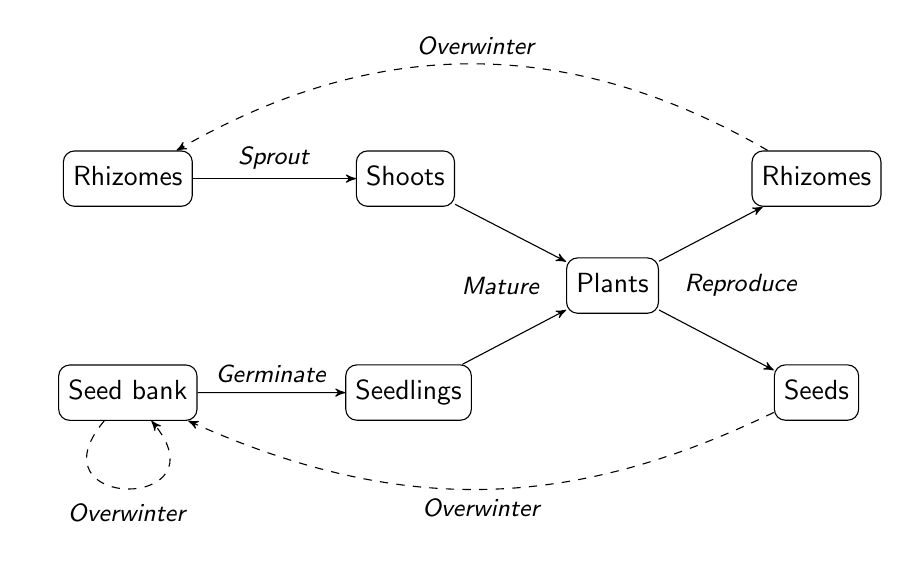
\begin{tikzpicture}[->,>=stealth']
	
	\node[state5] (PRIME) 
	{
		\begin{tabular}{c} 	
		Rhizomes\\
		\end{tabular}
	};
	
	\node[state5,  
	below=2.36cm of PRIME, 
	anchor=center] (BANK)
	{
		\begin{tabular}{c} 	
		Seed bank
		\end{tabular}
	};
	
	
	\node[state5,
	right= 2.7cm of PRIME,
	anchor=center] (TILLERS) 
	{
		\begin{tabular}{c}
		Shoots\\
		\end{tabular}
	};
	
	\node[state5,   
	below right= 1cm and 2cm of TILLERS, 
	anchor=center] (PLANTS)
	{
		\begin{tabular}{c} 	
		Plants\\
		\end{tabular}
	};
	
	\node[state5,  
	below left=1cm and 2cm of PLANTS, 
	anchor=center] (SEEDLINGS)
	{
		\begin{tabular}{c} 	
		Seedlings
		\end{tabular}
	};
	
	\node[state5,    
	above right=1cm and 2cm of PLANTS, 
	anchor=center] (TERT)
	{
		\begin{tabular}{c} 	
		Rhizomes\\
		\end{tabular}
	};
	
	\node[state5,  
	below right=1cm and 2cm of PLANTS, 
	anchor=center] (SEEDS)
	{
		\begin{tabular}{c} 	
		Seeds
		\end{tabular}
	};
	
	
	\node[left=0.2cm of PLANTS, 
	anchor=east]{ \small \textit{Mature}};
	\node[right=0.2cm of PLANTS, 
	anchor=west]{{\small\textit{Reproduce}}};
	
	\path 
	(BANK) edge node[anchor=south,above]{{\small\textit{Germinate}}} (SEEDLINGS)
	(PRIME) edge node[anchor=south,above]{{\small\textit{Sprout}}} (TILLERS)
	(TILLERS) edge (PLANTS)
	(SEEDLINGS) edge (PLANTS)
	(PLANTS) edge (TERT)
	(PLANTS) edge (SEEDS)
	(TERT) edge[style={dashed}, bend right=30] node[anchor=south,above]{{ \small \textit{Overwinter}}} (PRIME)
	(SEEDS) edge[style={dashed}, bend left=25] node[anchor=north,below]{{\small\textit{Overwinter}}} (BANK)
	(BANK) edge[style={dashed}, loop below,out=270-40, in=270+40, distance=15mm] node[anchor=north,below]{\begin{tabular}{r}
		{\small\textit{Overwinter}}
		\end{tabular}} (BANK);
	
	\end{tikzpicture}
	
\end{document}